\chapter{Конструкторская часть}

В данном разделе будут приведены схемы алгоритмов нахождения расстояний Левенштейна и Дамерау-Левенштейна, приведено описанию используемых типов данных, оценки памяти, а также описана структура ПО.

\section{Разработка алгоритмов}

На вход алгоритмов подаются строки $S_1$ и $S_2$

На рисунке \ref{fig:Liter} представлен схема алгоритма поиска расстояния Левенштейна.

На рисунках \ref{fig:DLiter} - \ref{fig:DLrechash2} представлены схемы алгоритмов поиска Дамерау-Левенштейна.

\begin{figure}[h]
	\centering
	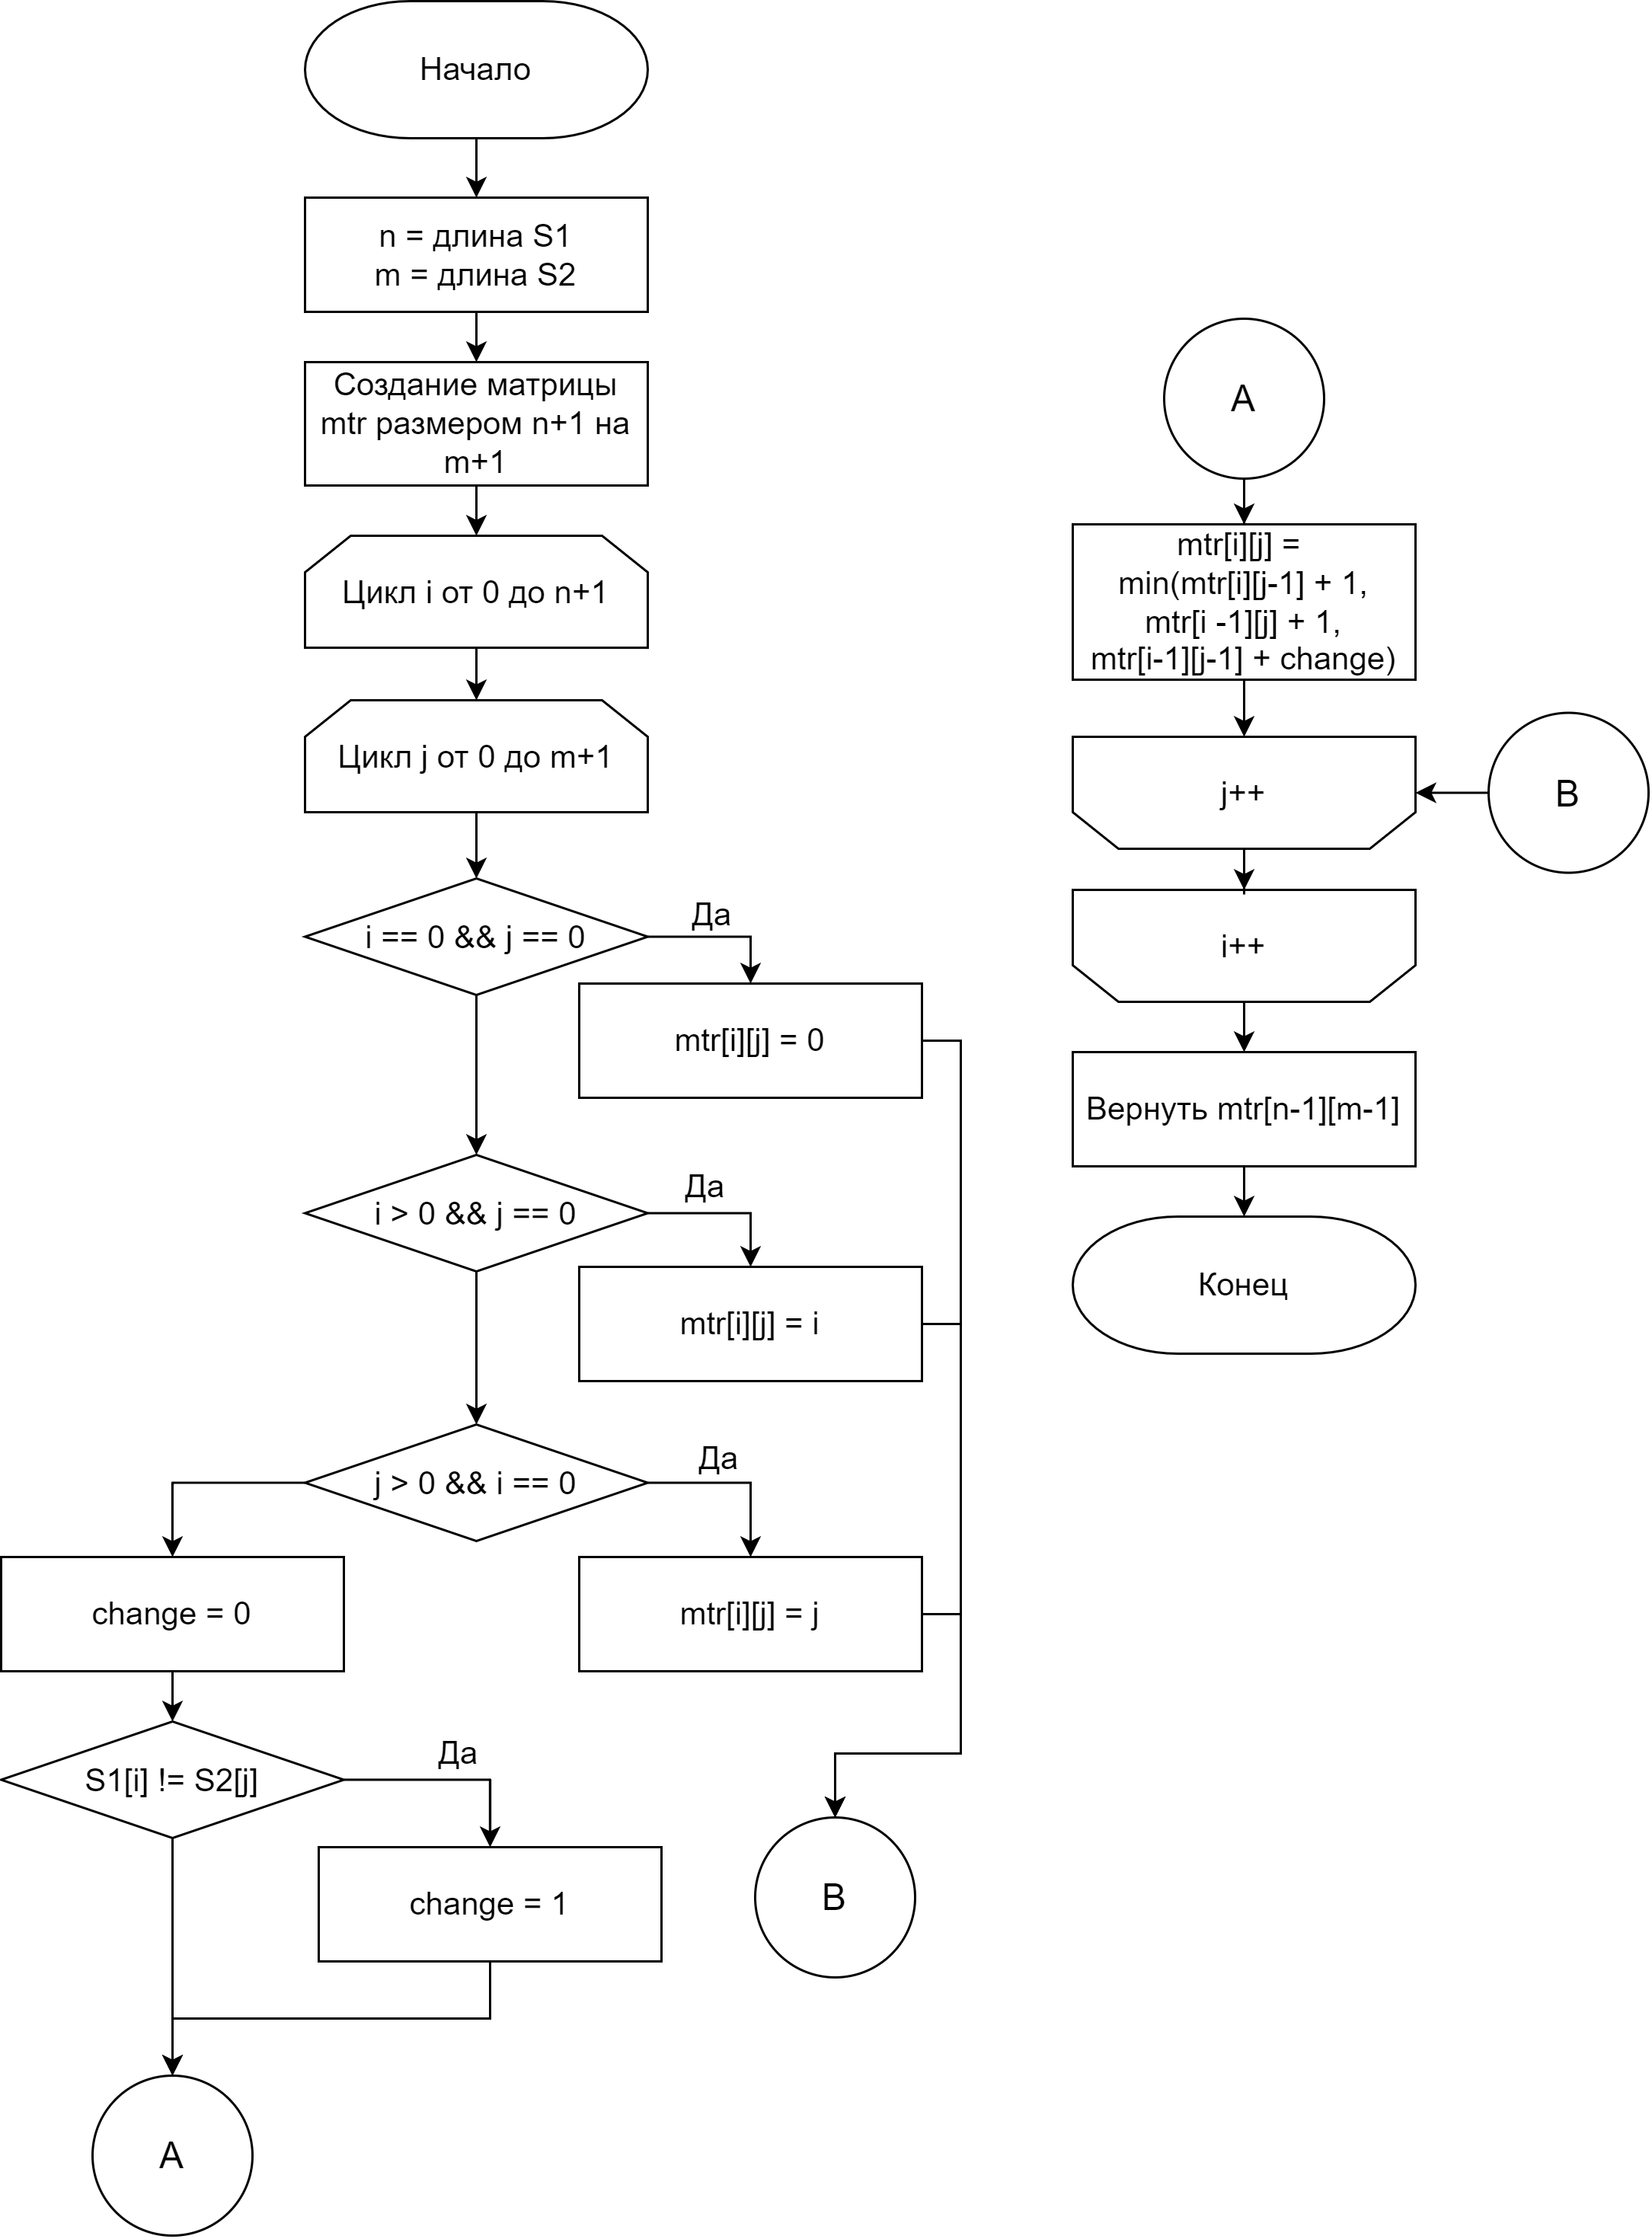
\includegraphics[height=0.8\textheight]{img/levmatr.png}
	\caption{Схема нерекурсивного алгоритма нахождения расстояния Левенштейна}
	\label{fig:Liter}
\end{figure}

\clearpage

\begin{figure}[h]
	\centering
	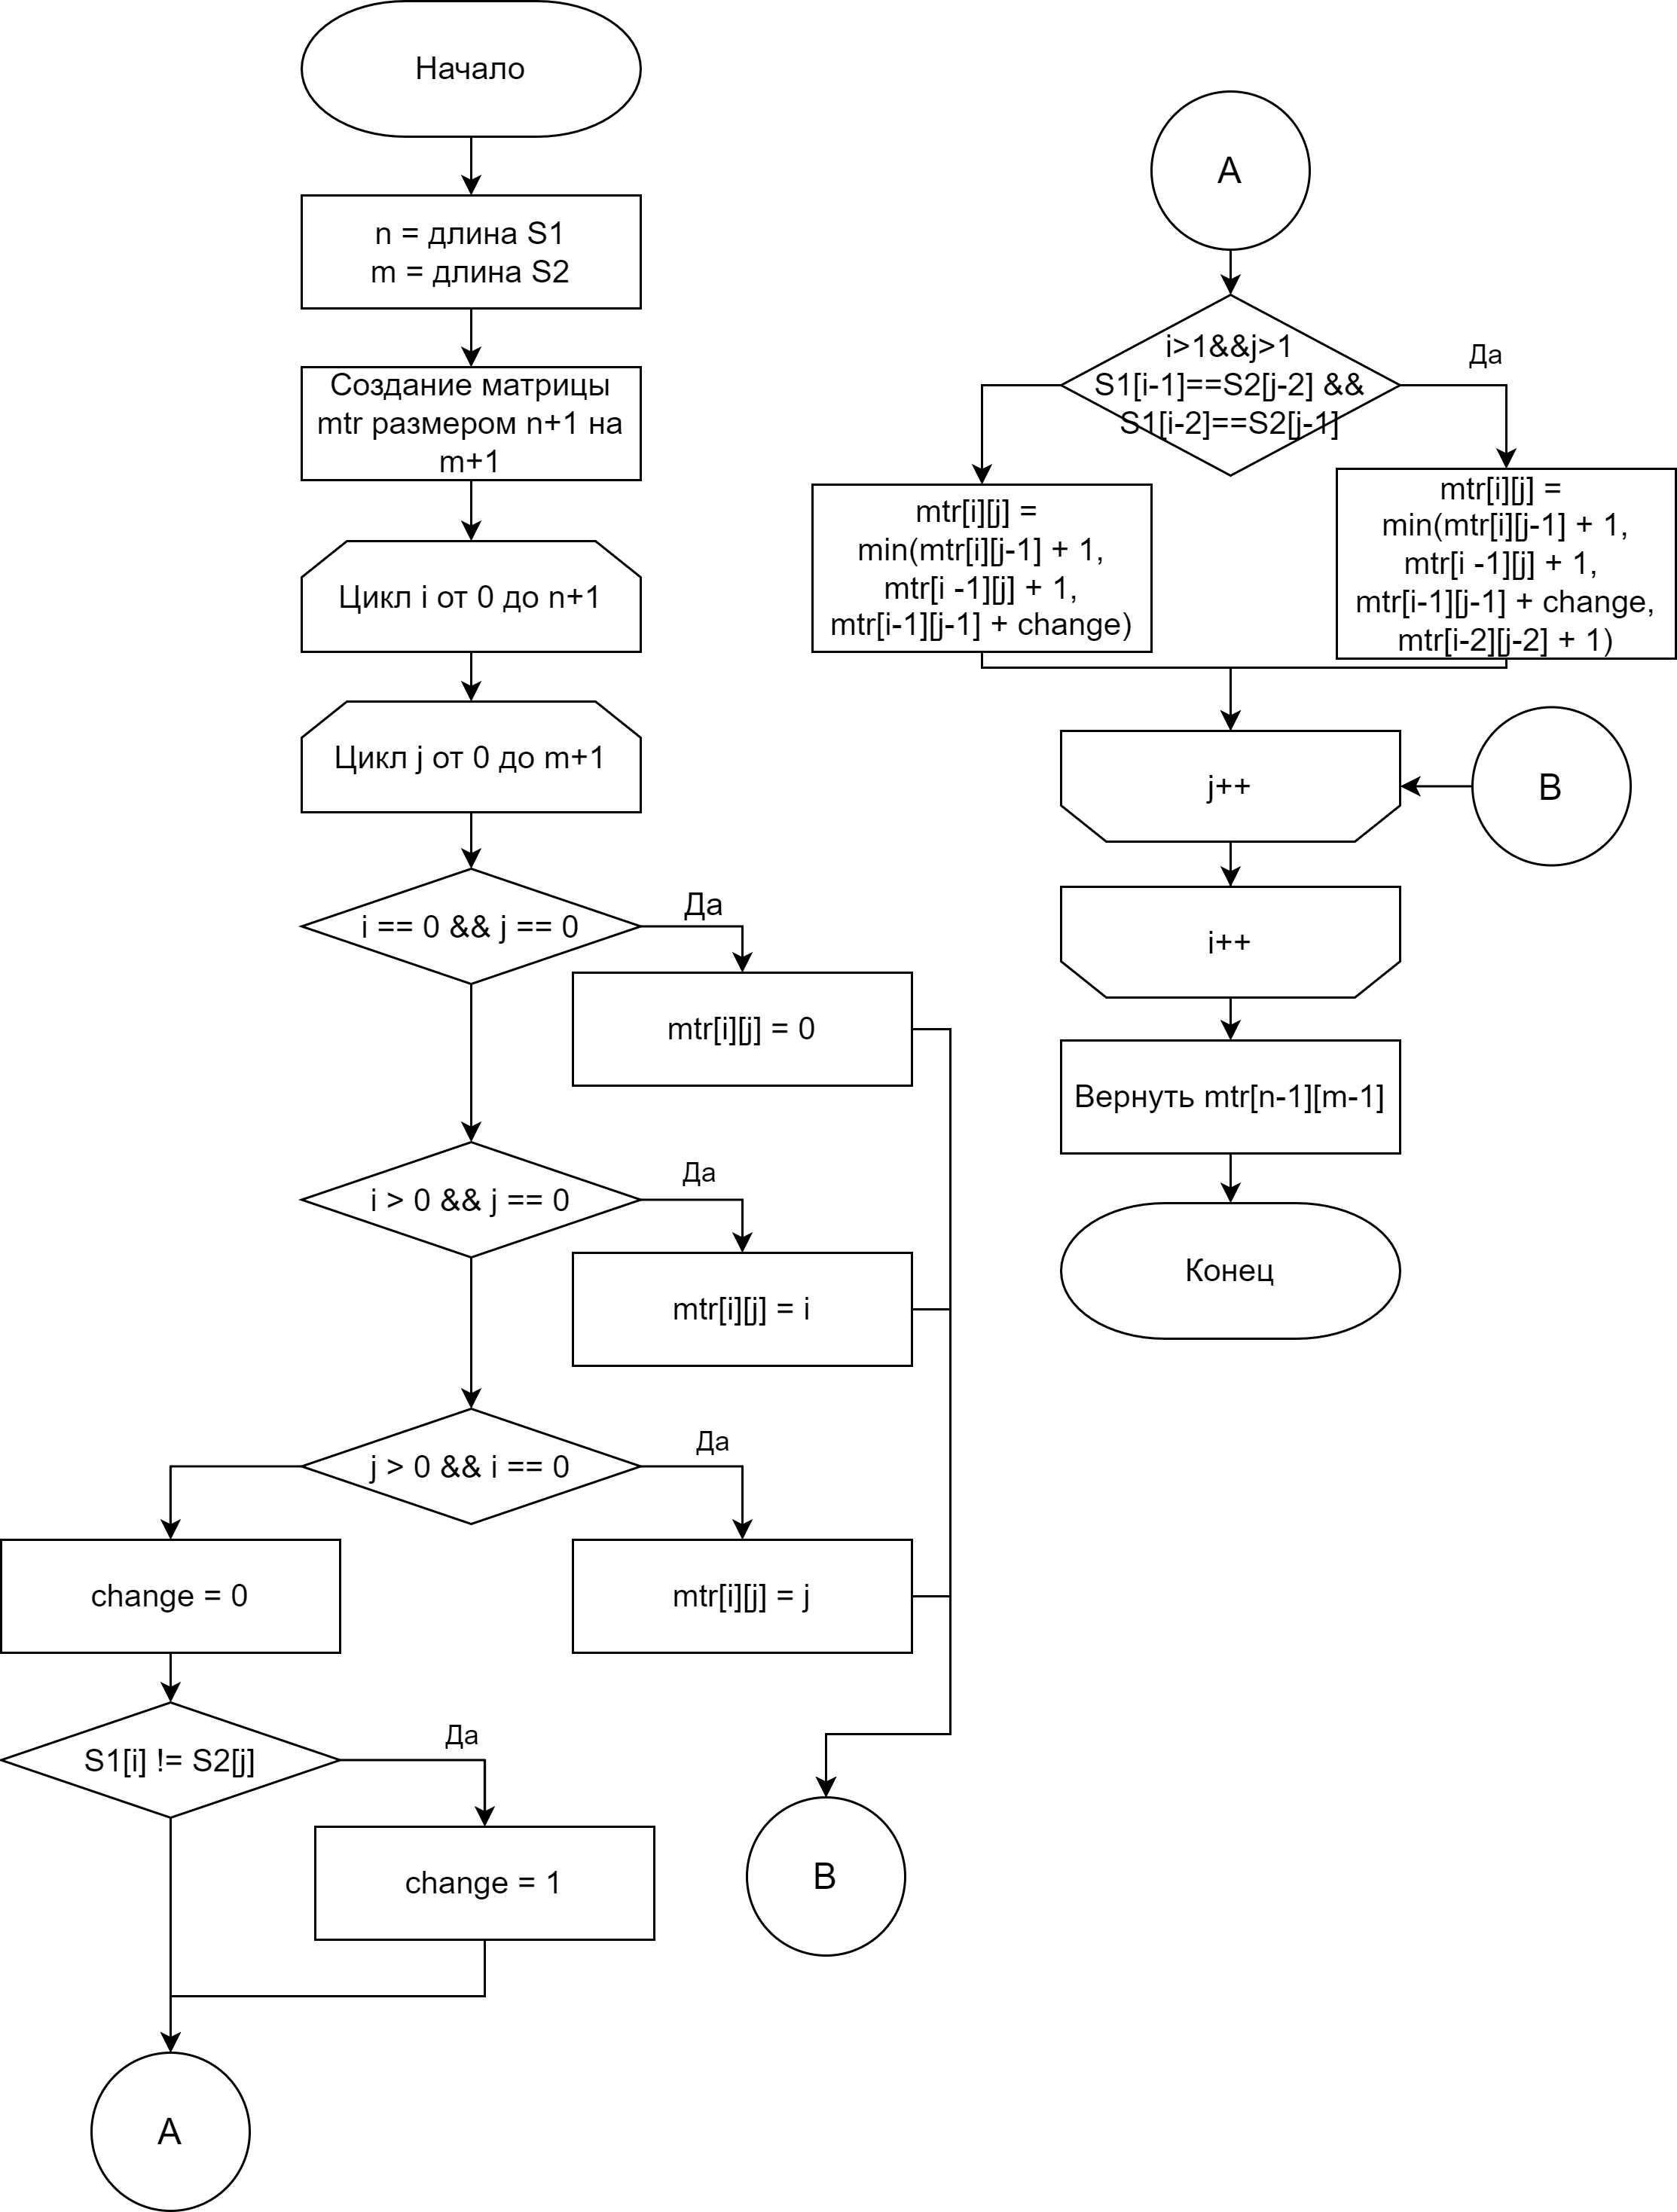
\includegraphics[height=0.8\textheight]{img/dliter.png}
	\caption{Схема нерекурсивного алгоритма нахождения расстояния Дамерау-Левенштейна}
	\label{fig:DLiter}
\end{figure}

\clearpage

\begin{figure}[h]
	\centering
	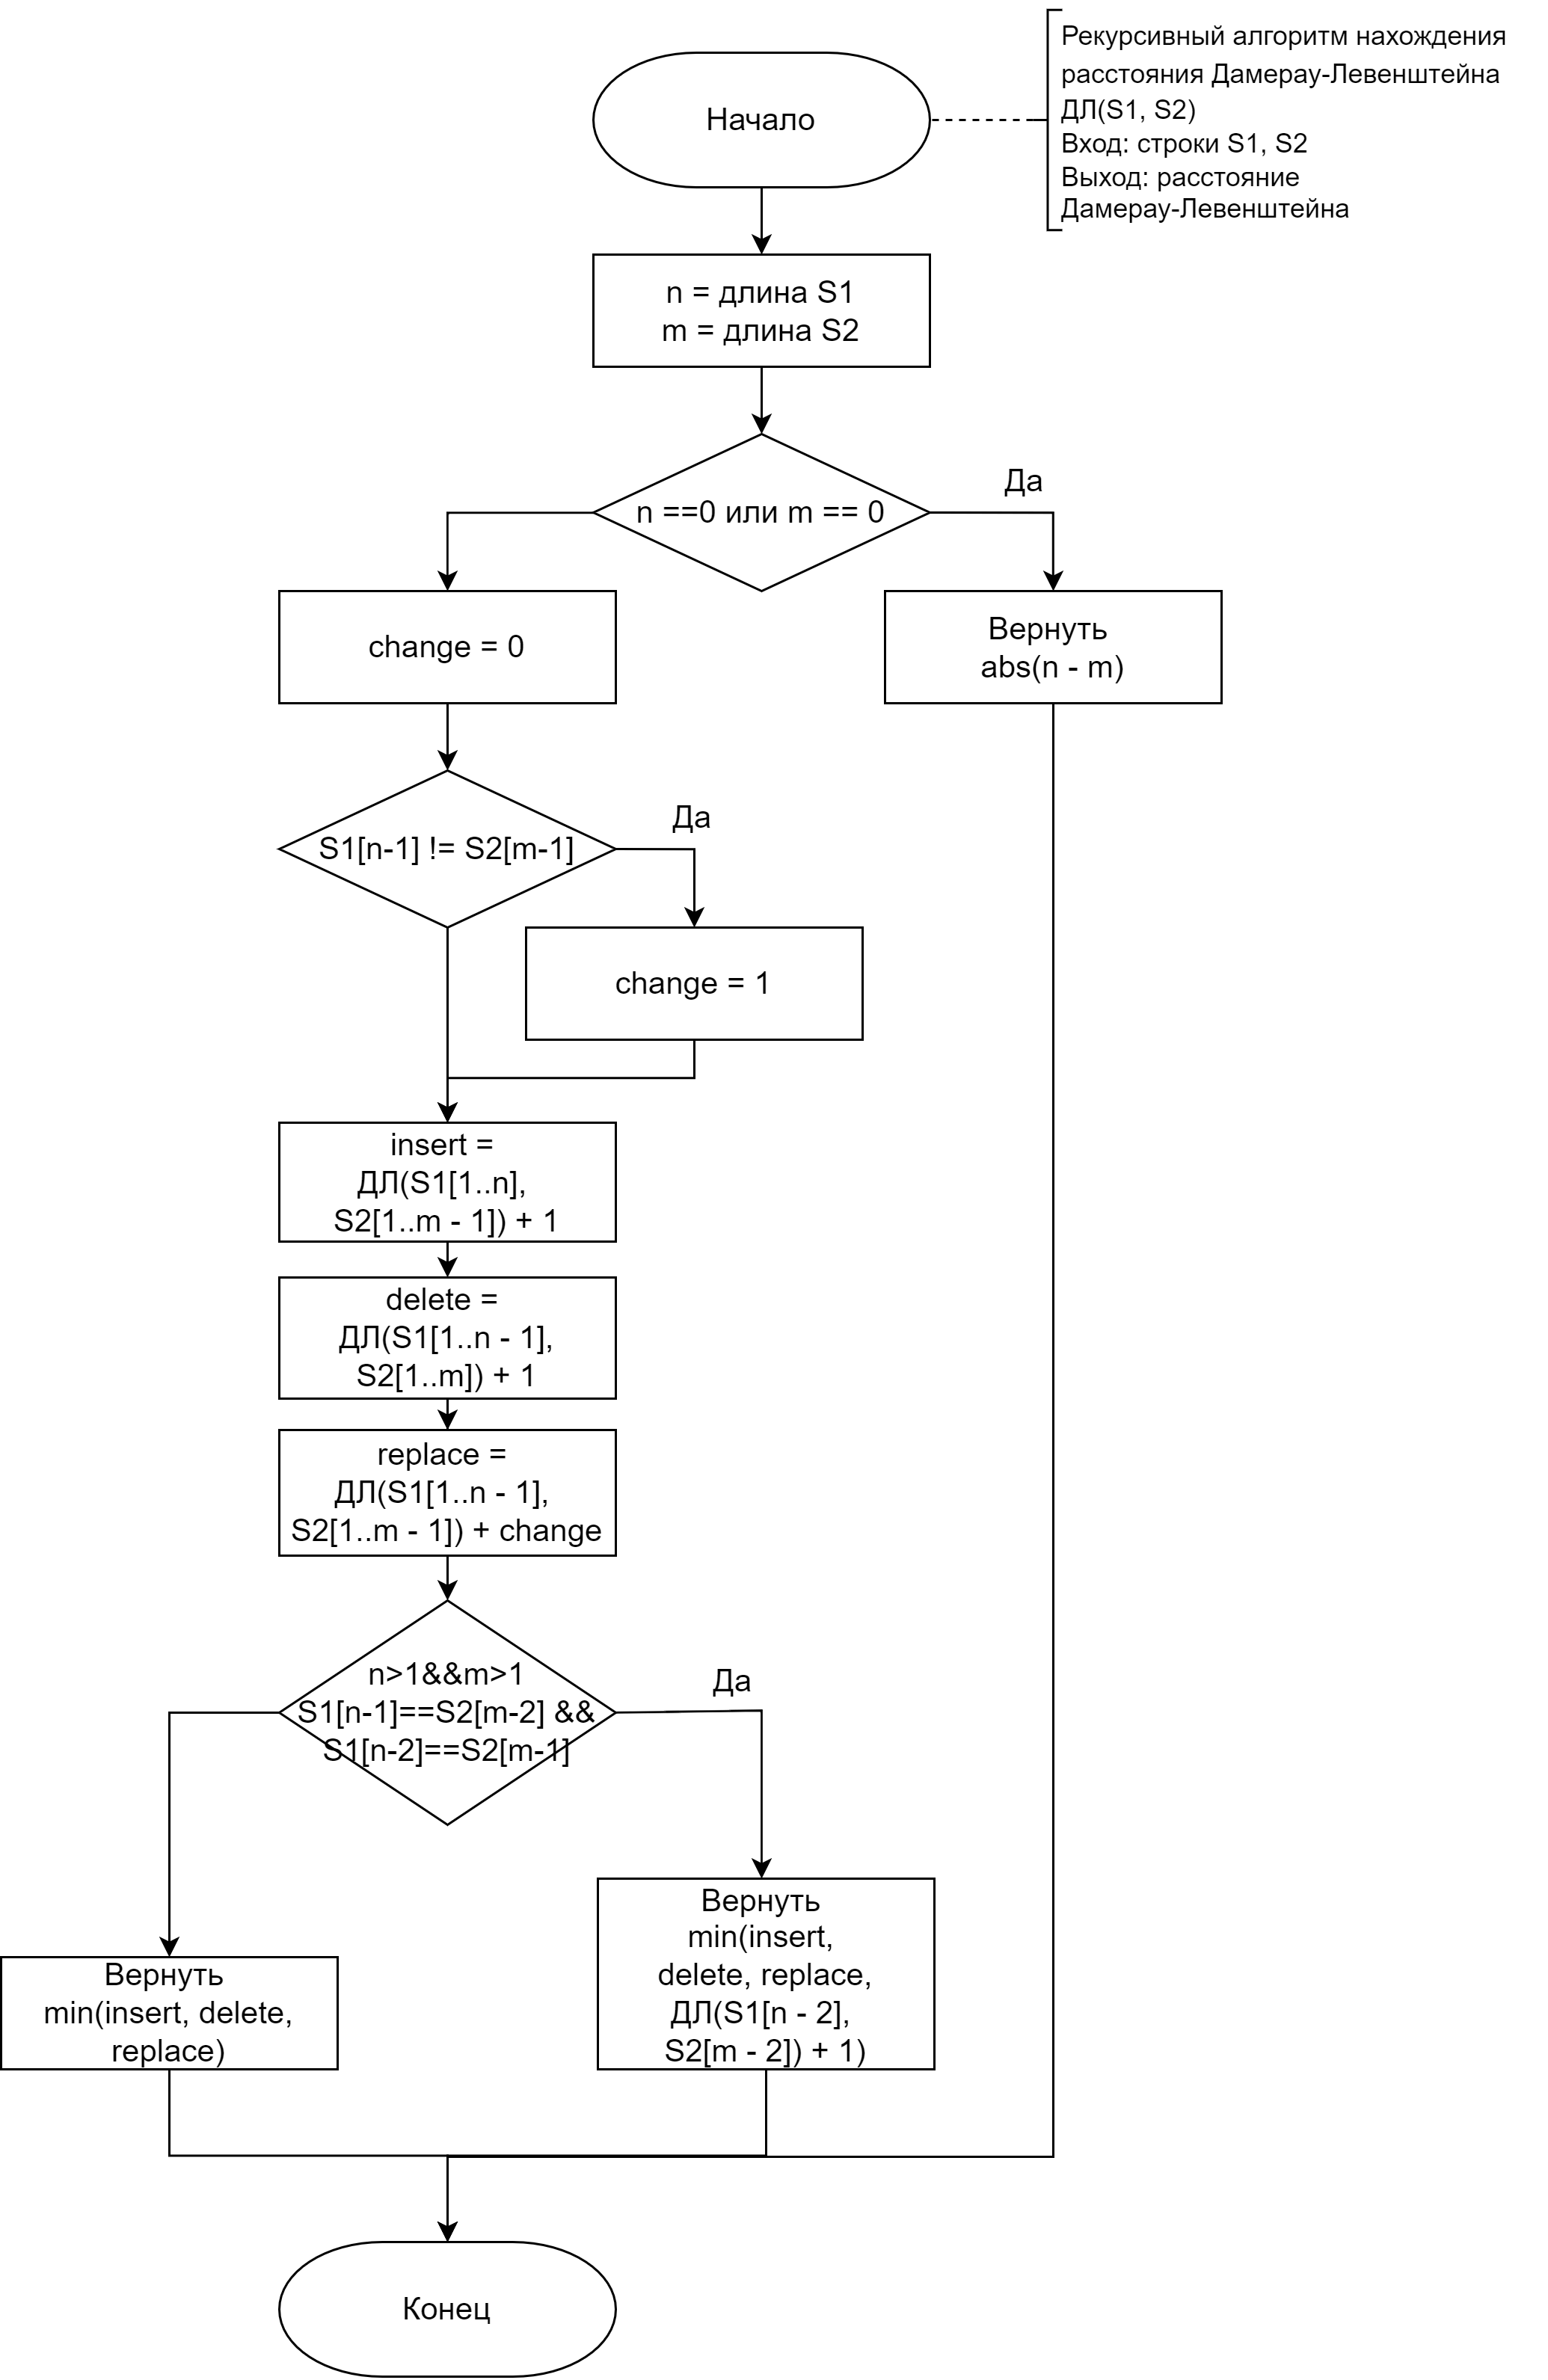
\includegraphics[height=0.8\textheight]{img/dlrec.png}
	\caption{Схема рекурсивного алгоритма нахождения расстояния Дамерау-Левенштейна}
	\label{fig:DLrec}
\end{figure}

\clearpage

\begin{figure}[h]
	\centering
	
\includegraphics[height=0.6\textheight]{img/dlrechash-1.png}
	\caption{Схема рекурсивного алгоритма нахождения расстояния Дамерау-Левенштейна с кешированием}
	\label{fig:DLrechash1}
\end{figure}

\clearpage

\begin{figure}[h]
	\centering
	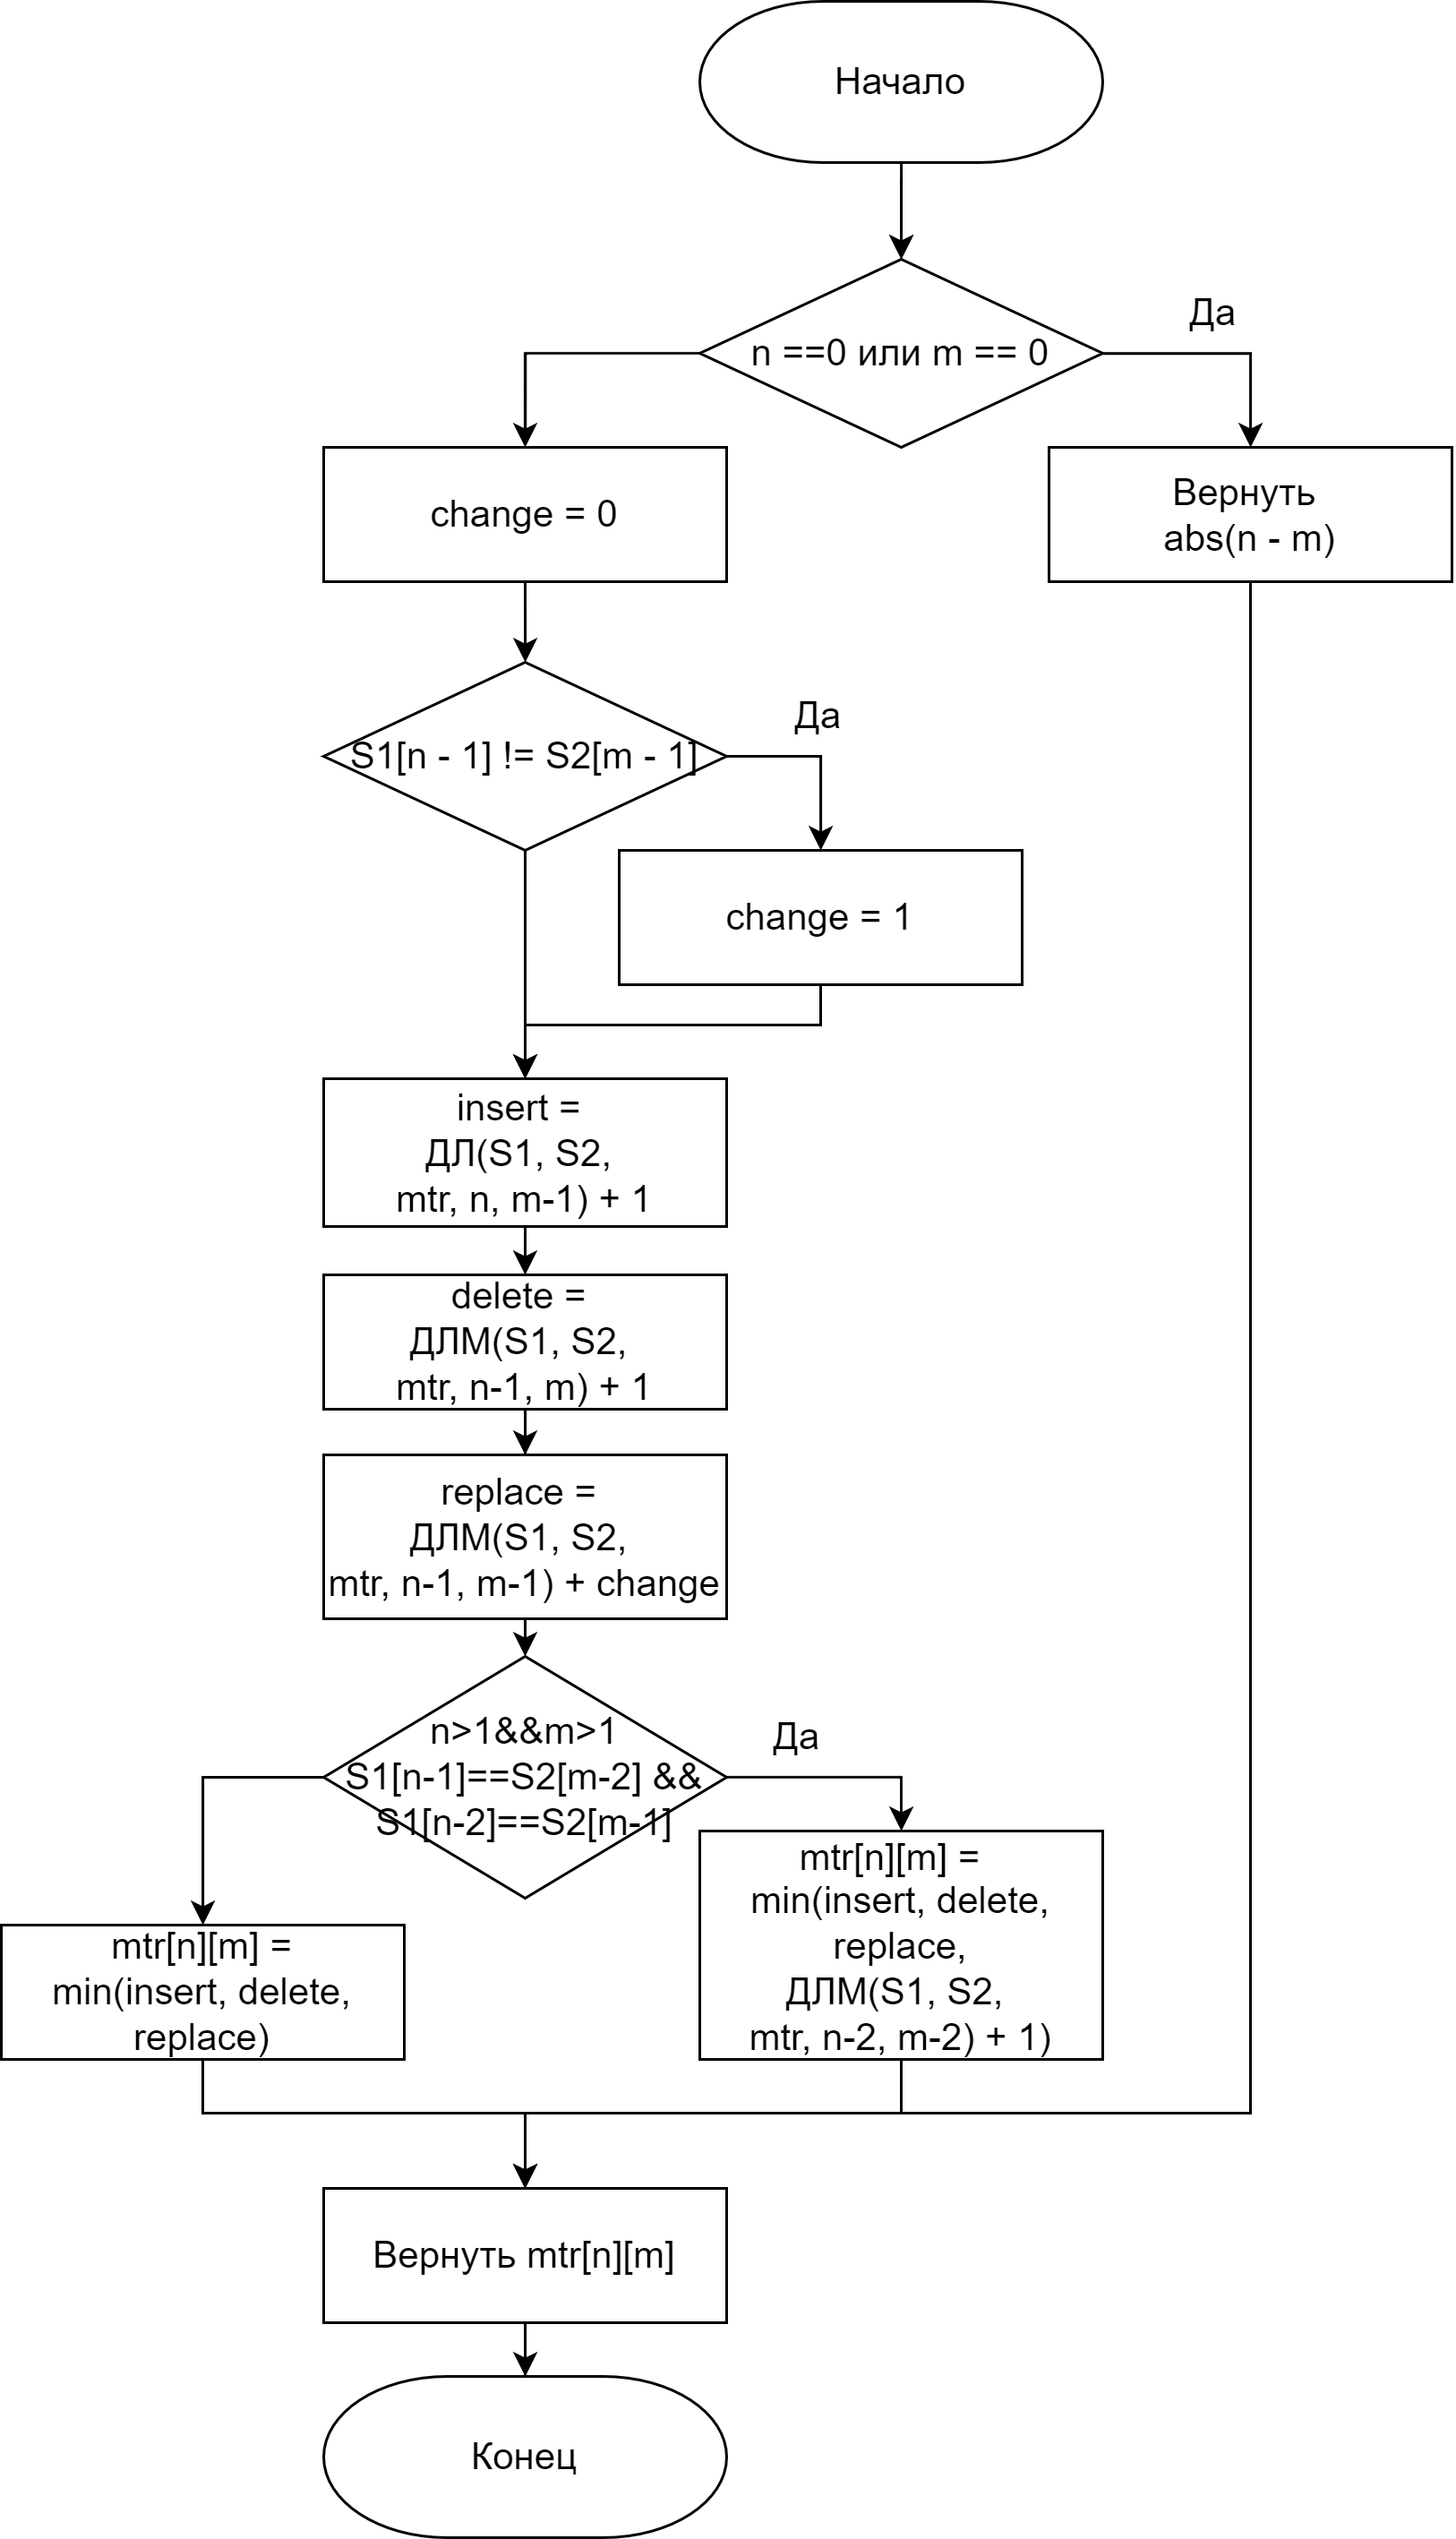
\includegraphics[height=0.8\textheight]{img/dlrechash-2.png}
	\caption{Схема алгоритма рекурсивного заполнения матрицы расстоянием Дамерау-Левенштейна}
	\label{fig:DLrechash2}
\end{figure}

\clearpage

\section{Описание используемых типов данных}

При реализации алгоритмов будут использованы следующие структуры данных:

\begin{itemize}
	\item строка - массив типа $char$ размером длины строки;
	\item длина строки - целое число типа $int$;
	\item матрица - двумерный массив типа $int$.
\end{itemize}

\section{Вывод}

В данном разделе на основе теоретических данных были построены схемы
требуемых алгоритмов, выбраны используемые типы данных.